\documentclass[11pt]{article}
\usepackage[margin=1in]{geometry}
\usepackage[expansion=false]{microtype}
\usepackage{hyperref}
\usepackage{xcolor}
\hypersetup{colorlinks=true, linkcolor=blue!60!black, citecolor=teal,
  urlcolor=blue!60!black}
\usepackage{graphicx}
\usepackage{booktabs}
\usepackage{amsmath, amssymb}
\usepackage{listings}
\usepackage{enumitem}
\usepackage{tikz}
\usetikzlibrary{positioning, arrows.meta, shapes.geometric, shapes.misc,
  backgrounds, fit, calc, decorations.pathreplacing}
\usepackage{float}
% Lightweight algorithm float — avoids the heavier algorithm/algpseudocode
% packages whose default styling clashes with our tabular-style listing.
\newfloat{algorithm}{htbp}{loa}
\floatname{algorithm}{Algorithm}
\setlist{itemsep=1pt, topsep=2pt}

% TBD macro for unfilled experiment cells
\newcommand{\TBD}[1]{%
  \textcolor{red!80!black}{\textsf{[TBD: #1]}}}

\title{\bfseries Memory as a Learned Policy:\\
\large Budgeted Write Operations for Long-Horizon LLM Agents}
\author{Parth Kocheta\\\small University of Maryland}
\date{\today}

\begin{document}
\maketitle

\begin{abstract}
Long-running language-model agents accumulate context faster than any
context window can hold, so they store some of it externally. Every
published memory system---Mem0, Letta, Mastra, Zep, our own
KGmem---decides what to commit using hand-written prompts and
heuristics. We ask whether the same decisions can be made by a learned
policy supervised by downstream answer correctness, the same signal
already used to evaluate the system.

Memory becomes a budgeted decision problem. Under a hard retention
budget $K$, a write policy emits a short sequence of typed operations
(\texttt{create\_entity}, \texttt{update\_state}, \texttt{add\_relation},
\texttt{mark\_contradiction}, \texttt{forget}, and others) into a
typed-transition knowledge graph; a fixed hybrid retriever fuses BM25,
dense, and named-entity lookups for the read side. The technical
obstacle is credit assignment: the policy emits four to twelve tokens
of tool calls per turn, but the reward only arrives later, when a
held-out question gets answered well or badly. Concurrent memory-RL
work (Memory-R1, Mem-$\alpha$) feeds GRPO a single trajectory-level
scalar that diffuses uniformly over those tokens; per-op resolution is
lost.

We propose \emph{per-op counterfactual marginal utility}. For each
mutating op $a_i$ in a write trajectory, we replay the trajectory
without it and measure how the held-out QA judge score changes. The op
gets credit equal to the difference. The trajectory reward GRPO sees is
the sum of these per-op deltas, but each op now carries its own
signal at advantage time. Lookups and noops are skipped --- their
effect on the post-write graph is zero by construction --- which keeps
the cost at roughly $5\times$ a trajectory-level signal in exchange
for per-op resolution. The technique is the COMA cooperative-RL
baseline applied at the granularity our typed op vocabulary makes
natural; the closest concurrent memory-RL work that gives op-level
rewards (DeltaMem) uses a state-distance signal, not an
outcome-attribution one.

The success criterion is strict. A learned write policy must beat
random subsampling at matched retention budget --- the content-agnostic
efficiency frontier --- and a BM25 heuristic that picks turns by query
overlap, on both LoCoMo and LongMemEval-S. \TBD{Headline numbers fill
in once the Phase~B run lands.}

Facts live in the store, strategy lives in the weights. The store
holds whatever the user gives it; the strategy transfers without
moving any of their data.
\end{abstract}

% --------------------------------------------------------------------------
\begin{figure}[t]
\centering
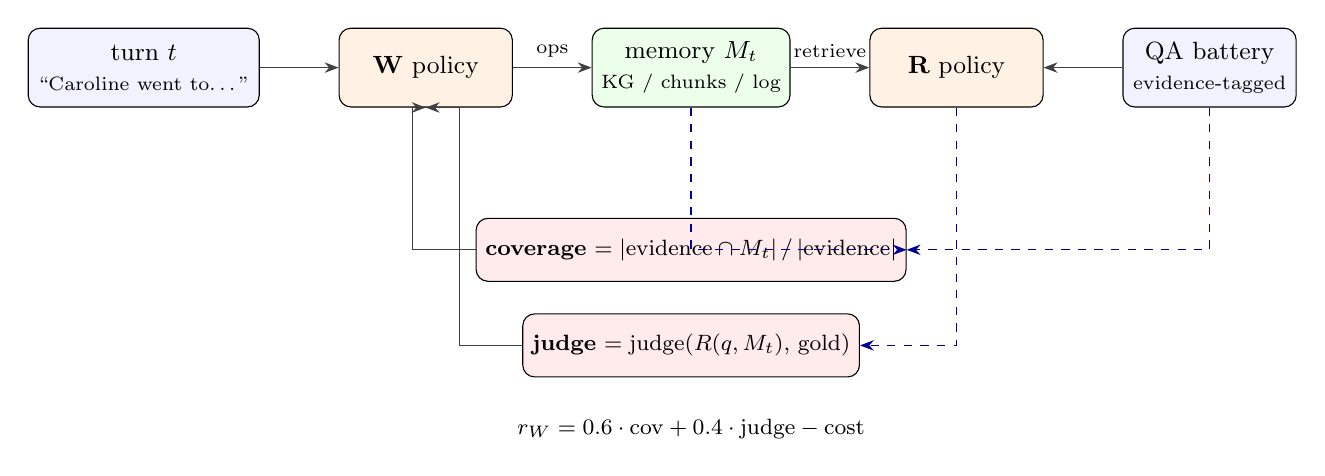
\begin{tikzpicture}[
  node distance=10mm,
  font=\small,
  conv/.style={draw, fill=blue!5, rounded corners=1.5mm, minimum width=22mm,
               minimum height=10mm, align=center, line width=0.4pt},
  policy/.style={draw, fill=orange!10, rounded corners=1.5mm,
                 minimum width=22mm, minimum height=10mm, align=center,
                 line width=0.4pt},
  store/.style={draw, fill=green!8, rounded corners=1.5mm,
                minimum width=22mm, minimum height=10mm, align=center,
                line width=0.4pt},
  reward/.style={draw, fill=red!8, rounded corners=1.5mm,
                 minimum width=42mm, minimum height=8mm, align=center,
                 line width=0.4pt, font=\footnotesize},
  arr/.style={-Stealth, line width=0.45pt, draw=black!75},
  flow/.style={-Stealth, line width=0.45pt, draw=blue!60!black, dashed},
]
\node[conv] (turn)  {turn $t$\\\scriptsize ``Caroline went to\dots''};
\node[policy, right=of turn] (W) {\textbf{W} policy};
\node[store, right=of W] (M) {memory $M_t$\\\scriptsize KG / chunks / log};
\node[policy, right=of M] (R) {\textbf{R} policy};
\node[conv, right=of R] (qa) {QA battery\\\scriptsize evidence-tagged};
\node[reward, below=14mm of M] (cov) {\textbf{coverage} $=
  |\text{evidence}\cap M_t|\,/\,|\text{evidence}|$};
\node[reward, below=4mm of cov] (judge) {\textbf{judge} $=
  \mathrm{judge}(R(q, M_t),\,\text{gold})$};
\node[draw=none, below=4mm of judge, font=\footnotesize\itshape]
  (rwd) {$r_W = 0.6\cdot\mathrm{cov} + 0.4\cdot\mathrm{judge} - \mathrm{cost}$};
\draw[arr] (turn)   -- (W);
\draw[arr] (W)      -- node[above, font=\scriptsize]{ops}      (M);
\draw[arr] (M)      -- node[above, font=\scriptsize]{retrieve} (R);
\draw[arr] (qa)     -- (R);
\draw[flow] (M.south) |- (cov.east);
\draw[flow] (R.south) |- (judge.east);
\draw[flow] (qa.south) |- (cov.east);
\draw[arr]  (cov.west) -- ++(-8mm,0) |- (W.south);
\draw[arr]  (judge.west) -- ++(-8mm,0) |- (W.south);
\end{tikzpicture}
\caption{The write policy~$W$ ingests one conversation turn and emits
memory ops; the read policy~$R$ later retrieves from the resulting store
$M_t$ to answer questions. $W$'s reward blends a deterministic
\emph{evidence-coverage} term against LoCoMo's per-question dia\_id labels
with an LLM-judge term over $R$'s answer. Coverage is dense and free;
judge keeps the policy honest about whether the stored content is
actually answerable.}
\label{fig:overview}
\end{figure}

\section{Introduction}

\paragraph{The problem in one sentence.} Long-running AI assistants
need long-running memory; today every system that does this in
production hand-codes the decision of what to write down. Mem0 prompts
an LLM to choose between \texttt{ADD/UPDATE/DELETE/NOOP} on each new
turn~\cite{chhikara2024mem0}. Letta moves items between three OS-style
memory tiers via prompted function calls~\cite{zhang2024memgpt}. Zep
maintains a knowledge graph whose edges expire under hand-written
rules~\cite{rasmussen2024zep}. Mastra runs two background LLM agents
(\emph{Observer} and \emph{Reflector}) that compress raw turns into a
bullet log on a fixed schedule and reach $94.87\%$ on LongMemEval with
GPT-5-mini~\cite{mastra2025om}. KGmem, the prior-art typed-transition
graph from the lead author that we use as one of our three backends,
resolves new mentions against existing entities via a three-tier
string/embedding/LLM cascade with thresholds chosen by inspection.
Each of these works in practice. Each is also a place where the
control logic is frozen --- the system cannot improve from the same
signal that was used to evaluate it.

\paragraph{Why hand-coding is fragile.} A prompt cannot adapt to one
user's writing style without being rewritten. A threshold cannot tell
that a particular conversation has many proper nouns and few facts,
or the reverse. A static rule cannot learn from its own mistakes:
when Mem0 fails to extract a fact (the Mem0 paper itself reports a
$\sim 40\%$ extraction-failure rate), the system has no way to
attribute the failure or update the rule. The recent Memory-R1 work
\cite{memoryR1} answers this by training a memory manager with
reinforcement learning end-to-end on QA accuracy. Mem-$\alpha$
\cite{memalpha2025} and DeltaMem~\cite{deltamem2026} extend the same
idea with richer memory ontologies and longer episode horizons.
The direction is right; the open question is the shape of the reward
that turns ``the agent answered well'' into a useful gradient on
``which write op deserved the credit?''

\paragraph{The credit-assignment problem, made concrete.} A write
policy that ingests one conversation turn typically emits two to four
tool calls --- maybe a \texttt{lookup\_entity} to check whether
``Caroline'' already exists, then a \texttt{create\_entity} that adds
her, then an \texttt{add\_relation} that links her to the LGBTQ support
group she mentioned, then a \texttt{noop} on the next turn that's just
a greeting. After this, future questions get asked. The reader
retrieves from whatever the write policy left behind and tries to
answer. The judge returns one number per question. GRPO~\cite{shao2024deepseekmath},
the standard critic-free RL algorithm for this kind of training, takes
the trajectory's reward and applies it as a uniform advantage to every
emitted token. So the four-token \texttt{create\_entity} call and the
four-token \texttt{noop} get the same gradient signal, despite making
opposite contributions to the answer. This is the diffuse-credit
problem and concurrent memory-RL work runs into it directly: Memory-R1
uses final-answer EM as a single per-trajectory scalar; Mem-$\alpha$
pools accuracy across an entire dialogue.

\paragraph{Our solution.} We propose \emph{per-op counterfactual
marginal utility}. For each mutating op $a_i$ the policy emitted, we
replay the trajectory without it, run the same reader against the
counterfactual memory state, and ask the judge whether each held-out
question still gets answered. The op's credit is the average drop in
judge score it would have caused by being absent. Lookups and noops
are skipped because their effect on the post-write graph is zero by
construction; only the mutating ops get attribution. The trajectory
reward GRPO sees is the sum of per-op deltas, but each op now
contributes its own credit signal at advantage time. The technique is
the COMA counterfactual baseline from cooperative multi-agent RL
\cite{foerster2018coma} applied at the op granularity our typed
vocabulary makes natural. The closest concurrent memory-RL work that
gives op-level rewards is DeltaMem~\cite{deltamem2026}, which uses a
state-distance signal (Memory-Levenshtein); ours is the first
outcome-attribution variant in this setting.

\paragraph{Why this matters.} The framing has two payoffs. For
research, it makes memory a \emph{learned operating system} ---
strategy in the weights, facts in the store --- with a backend-agnostic
op vocabulary that compiles to three different storage substrates we
test. For deployment, the same property gives a useful asymmetry: a
single trained adapter can run against any user's local store, no
per-user fine-tuning, no need to move user data into a shared corpus.
The store holds whatever the user gives it; the strategy transfers
without moving any of their data.

\paragraph{Contributions.}
\begin{enumerate}
  \item A reframing of LLM-agent memory as a \emph{budgeted decision
    problem}: under a hard retention budget $K_{\max}$, the learnable
    layer is the write policy that picks which $K$ items to commit.
    Read becomes a hand-coded hybrid retrieval stack that the write
    policy optimises against.
  \item \textbf{Per-op counterfactual marginal utility} as the dense
    write reward for memory-RL GRPO. Adapted from the COMA cooperative
    multi-agent baseline; novel in the memory-write setting, where
    concurrent work uses either trajectory-level outcome rewards
    (Memory-R1, Mem-$\alpha$) or state-distance per-op rewards
    (DeltaMem) that don't directly say what the downstream reader
    needs.
  \item A backend-retriever-aligned evaluation protocol that controls
    for the dominant confound in memory-system comparison: a paired
    LoCoMo audit shows mismatched retrievers can swing QA accuracy by
    $0.40$ in absolute terms (McNemar $p = 1.9\!\times\!10^{-6}$). We
    run training and evaluation on the same hybrid retriever (BM25 +
    dense + NER fused with RRF).
  \item Two strict baselines the learned policy must beat: random
    subsampling at matched $F$ (the content-agnostic efficiency
    frontier) and a BM25 heuristic that picks turns by query overlap.
    We report area under the efficiency curve (AUEC) as the headline
    metric.
  \item Empirical results on LoCoMo and LongMemEval-S, plus a
    head-to-head against KGmem's hand-coded extraction on personal
    ChatGPT-export data with self-generated questions
    (Section~\ref{sec:eval-modes} Mode~C). \TBD{Numbers fill in once
    the long Phase~B run completes.}
\end{enumerate}

Figure~\ref{fig:overview} shows the data-flow once. The rest of the
paper goes through the parts in order: related work in
\S\ref{sec:related}, the op vocabulary and reward in \S\ref{sec:method},
benchmarks and baselines in \S\ref{sec:exp-main}, and a discussion of
what we believe and what we don't in \S\ref{sec:discussion}.

% --------------------------------------------------------------------------
\section{Related Work}
\label{sec:related}

The right way to navigate the memory-systems literature is along two
orthogonal axes: where do the facts live, and where does the write
control come from. Table~\ref{tab:landscape} places each major system on
the grid; the cell we sit in (external store, learned ops) is also the
smallest and the most recently populated.

\begin{table}[h]
\centering
\small
\caption{The memory-systems design grid. Rows are storage substrate;
  columns are how the write decisions are made. The published memory-RL
  cluster (right column) all use trajectory-level outcome rewards
  except DeltaMem (state-distance) and ours (per-op outcome
  attribution).}
\label{tab:landscape}
\begin{tabular}{p{0.27\linewidth} p{0.32\linewidth} p{0.32\linewidth}}
\toprule
\textbf{Substrate} & \textbf{Hand-coded ops} & \textbf{Learned ops} \\
\midrule
Flat KV / chunk index   &
  Mem0~\cite{chhikara2024mem0}, naïve RAG & --- \\
Tiered OS-style memory  &
  Letta / MemGPT~\cite{zhang2024memgpt} & --- \\
Knowledge graph         &
  Zep / Graphiti~\cite{rasmussen2024zep}, KGmem &
  \textbf{this work}, DeltaMem~\cite{deltamem2026} \\
Observation / summary log &
  Mastra OM~\cite{mastra2025om}, Generative Agents~\cite{park2023generative} &
  Mem-$\alpha$~\cite{memalpha2025}, Memory-R1~\cite{memoryR1} \\
Model weights           &
  ROME / MEMIT~\cite{meng2022rome}, per-user fine-tuning,
  Cartridges~\cite{cartridges2025} & --- \\
Implicit (test-time recurrence) &
  Recursive Language Models~\cite{rlm2025},
  Titans~\cite{titans2025} & --- \\
\bottomrule
\end{tabular}
\end{table}

\subsection{The hand-coded column}

Most production systems live here. The pattern is uniform: a prompt
written by a researcher decides what to commit, sometimes with
heuristics that fire afterward. Mem0 and Letta cap retention by tier or
recency; Zep maintains valid-time intervals on KG edges; Mastra runs an
\emph{Observer} pass to extract candidate facts and a \emph{Reflector}
pass to compress the trail. Mastra's $94.87\%$ on LongMemEval with
GPT-5-mini is the strongest published number, but the cost is paid in
LLM calls at write time --- the Reflector runs on every conversation
chunk, regardless of whether the fact it extracts will ever be queried.
Mem0's own paper reports a $\sim 40\%$ extraction-failure rate, which
is the visible signature of the underlying issue: a hand-tuned prompt
can't tell which extractions matter for the answers users will
eventually ask. Generative Agents~\cite{park2023generative} run
periodic reflection cycles that condense observations into higher-level
beliefs by the same template. Recursive Language
Models~\cite{rlm2025} sit in a different cell entirely --- they do
no write-time work and instead use a test-time outer loop to decide
how deeply to decompress the input context per query. RLM with
Gemini 3 Flash hits $89.8\%$ on LongMemEval, a strong result that
suggests \emph{when to spend test-time compute on memory} may be as
important as \emph{what to commit}. We treat RLM as orthogonal: a
trained mempol write policy could be paired with an RLM-style read
loop, and the two contributions would compose.

\subsection{The learned-ops column}

Concurrent published work in this cell is small but growing.
\textbf{Memory-R1}~\cite{memoryR1} trains a Memory Manager (ADD,
UPDATE, DELETE, NOOP) and an Answer Agent jointly with PPO/GRPO on
$152$ QA pairs from LoCoMo, MSC, and LongMemEval; the reward is final
QA accuracy at the trajectory level. \textbf{Mem-$\alpha$}~\cite{memalpha2025}
uses a richer memory ontology (core, episodic, semantic) and reports
$13\times$ generalisation in horizon length (training at 30k tokens,
testing at 400k). \textbf{DeltaMem}~\cite{deltamem2026} is the closest
to ours: it gives op-level rewards via a Memory-based Levenshtein
Distance on the post-write state. The difference between DeltaMem's
reward and ours is exactly the difference between asking ``did the op
change the memory in a structured way?'' and ``did the op change what
the reader can answer?''. Both are reasonable. Ours is more directly
aligned with the downstream task; theirs is cheaper to compute.
The earlier non-RL precedents are \textbf{ACE}~\cite{ace2026} (evolves
text-form playbooks based on execution feedback, but the playbook is a
single prompt) and \textbf{Voyager}~\cite{wang2023voyager} (maintains a
Minecraft skill library, with the LLM deciding what to add by
trial-and-error rather than RL).

\subsection{The RL machinery we use}

\textbf{GRPO}~\cite{shao2024deepseekmath} is the critic-free
simplification of PPO that has become the default for tool-use
training. For each prompt, sample $G$ rollouts; the advantage of
rollout $i$ is $(r_i - \bar{r})/\mathrm{std}(r)$. The group acts as a
zero-bias baseline. This works well when reward is verifiable (math,
code, judge-graded QA) and is what we use.
\textbf{Search-R1}~\cite{jin2025searchr1} applies GRPO to multi-turn
search-then-answer; we use the Tinker-cookbook reproduction of
Search-R1 as the structural template for our environment.
\textbf{Reflexion}~\cite{shinn2023reflexion} and verbal-RL approaches
update natural-language self-reflections rather than weights; they are
fast and cheap but plateau because the policy is a static prompt.
\textbf{Curriculum learning}~\cite{bengio2009curriculum} appears here
because we use it on the read side: LoCoMo's question categories give
us a natural easy-to-hard ordering. \textbf{LoRA}~\cite{hu2021lora} is
the adapter form-factor; we use rank-32 on
Qwen3-4B-Instruct~\cite{tinker2025}, trained via Tinker.

\subsection{Temporal awareness as a separate axis}

A distinct cluster of recent work shows that LLM agents fail at
\emph{behaving in time} --- not at computing date arithmetic, but at
deciding when to act. \textbf{Temporally Blind}~\cite{tictoc2025}
introduces TicToc, a 76-scenario benchmark that scores agent decisions
about when to refetch stale context; the best model alignment with
human preferences is $65\%$. \textbf{Real-Time
Deadlines}~\cite{realtimedeadlines2026} shows GPT-5.1 closes $4\%$ of
deals in time-pressured negotiation without a clock-in-prompt and
$32\%$ with one. \textbf{Robotouille}~\cite{robotouille2025} reports a
$47\% \to 11\%$ collapse for ReAct agents the moment planning has to
interleave synchronous and asynchronous actions. These are
benchmarks of \emph{behaviour}, not benchmarks of date-arithmetic
(Test of Time~\cite{testoftime2024} and Time-R1~\cite{timer1_2025}
cover the latter, with synthetic curricula and dedicated three-stage
RL respectively). The TemporalBench we propose
in~\S\ref{sec:datasets} extends TicToc's single-axis scoring to six
axes of behaviour and is positioned squarely in this cluster.

\subsection{What's missing, and what we add}

Across the grid, no published system combines (i) discrete
interpretable memory ops, (ii) chosen by a policy trained with
outcome supervision, (iii) where the supervision attributes credit
\emph{per op} rather than per trajectory or per state-distance.
Memory-R1 and Mem-$\alpha$ have (i) and (ii) but not (iii); DeltaMem
has (i), (ii), and a per-op signal but the signal is state-distance,
not outcome-attribution. That is the gap we close.

% --------------------------------------------------------------------------
\section{Method}
\label{sec:method}

\subsection{The op vocabulary}

We define a unified action space $\mathcal{A} = \mathcal{A}_R \cup
\mathcal{A}_W$. Each action is a JSON tool call with a fixed schema.

\paragraph{Read ops $\mathcal{A}_R$.}
\begin{itemize}
  \item \texttt{memory\_search(query, k, source)}: Retrieve top-$k$ chunks
    by lexical (BM25), semantic (dense), or hybrid (RRF~\cite{shao2024deepseekmath})
    match. The retrieval substrate is whichever Backend the env was built
    with.
  \item \texttt{memory\_expand(seed\_uids, k\_per)}: Pull adjacent chunks
    of seeds (one-hop graph follow / sibling-turn lookup).
  \item \texttt{memory\_filter(predicate, value)}: Restrict the current
    hit set by session, speaker, or time window.
  \item \texttt{memory\_rerank(strategy, query)}: Re-order hits by dense
    similarity, recency, or session order.
\end{itemize}
The episode ends when the model emits a final answer formatted as
``\texttt{Answer: \ldots}''.

\paragraph{Write ops $\mathcal{A}_W$.}
\begin{itemize}
  \item \texttt{noop}: This turn is not memory-worthy. The default.
  \item \texttt{lookup\_entity(query, type, top\_k)}: Find existing
    entities by name. The policy uses this to avoid duplicates.
  \item \texttt{lookup\_relation(source\_uid, target\_uid)}: Inspect
    existing graph edges.
  \item \texttt{create\_entity(name, type, state)}: Add a new entity.
    Type is one of nine: \texttt{person}, \texttt{project}, \texttt{tool},
    \texttt{organization}, \texttt{belief}, \texttt{decision},
    \texttt{concept}, \texttt{period}, \texttt{event}, \texttt{goal}.
  \item \texttt{update\_state(uid, new\_state, transition\_type,
    trigger\_summary)}: Mutate an entity. Transition type is one of
    \texttt{update}, \texttt{contradiction}, \texttt{resolution},
    \texttt{archival}.
  \item \texttt{merge\_entities(canonical\_uid, alias\_uid)}: Collapse
    two entities, moving transitions and edges.
  \item \texttt{add\_relation(source\_uid, target\_uid, rel\_type,
    description)}: Add a typed graph edge.
  \item \texttt{mark\_contradiction(uid, contradicting\_state)}: Flag
    that the current turn conflicts with the entity's prior state, but
    do not pick a winner.
  \item \texttt{forget(uid, reason)}: Soft-delete (archive). Keeps the
    transition history but marks the entity inactive.
\end{itemize}

\subsection{Background: KGmem, a typed-transition knowledge graph}
\label{sec:pie}

One of the three backends we evaluate predates this paper. We refer to
it throughout as \emph{KGmem}; the open-source implementation is the
PIE memory system from prior work by the lead author, retained in our
repository under \texttt{pie/}. We use a renamed reference here for
readability and to keep the role of the data structure separate from
the role of any specific control layer.

KGmem represents the user's world as a graph of typed entities (one of
\texttt{person}, \texttt{project}, \texttt{tool}, \texttt{organization},
\texttt{belief}, \texttt{decision}, \texttt{concept}, \texttt{period},
\texttt{event}, or \texttt{goal}). Each entity carries a history of
typed state transitions: every transition records a $(\textit{from
state},\,\textit{to state})$ pair labelled with one of
\texttt{creation}, \texttt{update}, \texttt{contradiction},
\texttt{resolution}, or \texttt{archival}. In particular,
contradiction is a first-class transition rather than an overwrite---an
unusual choice among open knowledge-graph memory systems---which lets
both the conflicting and prior states coexist until a later transition
resolves them. KGmem also supports per-entity importance scoring and
typed relationship edges; this paper uses the entity-plus-transition
substrate only.

KGmem matters here for two reasons. First, the typed transitions give
the write policy a richer action vocabulary than ``store'' and
``delete''---it can emit \texttt{contradiction} when a turn conflicts
with an existing entity, leaving both states retrievable for the read
policy. Second, entity uids let the read policy chain queries
(\texttt{lookup\_entity} $\to$ \texttt{transitions\_for(uid)}) when a
question requires multi-hop reasoning over a single entity's evolving
state. We re-use the data structure; the hand-coded extraction prompts
and three-tier resolver that ship with KGmem are replaced by the
learned write policy.

\begin{figure}[h]
\centering
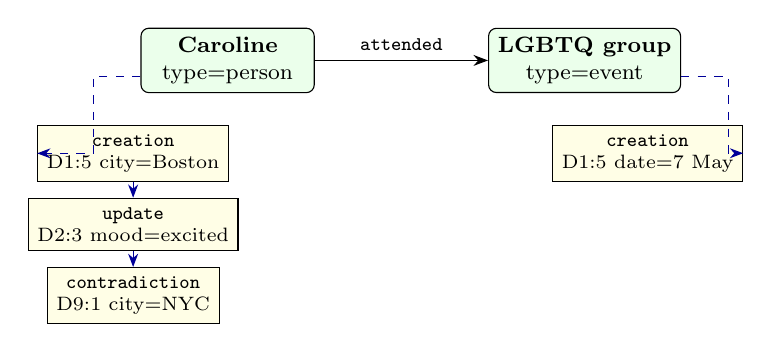
\begin{tikzpicture}[
  font=\footnotesize,
  ent/.style={draw, rounded corners=1mm, fill=green!8, minimum width=22mm,
              minimum height=8mm, align=center, line width=0.4pt},
  trans/.style={draw, fill=yellow!10, minimum width=18mm, minimum height=6mm,
                align=center, font=\scriptsize, line width=0.4pt},
  rel/.style={-Stealth, line width=0.5pt},
  evo/.style={-Stealth, line width=0.4pt, draw=blue!60!black, dashed},
  lab/.style={font=\scriptsize, midway},
]
\node[ent] (e1) {\textbf{Caroline}\\type=person};
\node[ent, right=22mm of e1] (e2) {\textbf{LGBTQ group}\\type=event};
\node[trans, below=4mm of e1, xshift=-12mm] (t1)
  {\texttt{creation}\\D1:5  city=Boston};
\node[trans, below=2mm of t1] (t2)
  {\texttt{update}\\D2:3  mood=excited};
\node[trans, below=2mm of t2] (t3)
  {\texttt{contradiction}\\D9:1  city=NYC};
\node[trans, below=4mm of e2, xshift=8mm] (t4)
  {\texttt{creation}\\D1:5  date=7~May};
\draw[rel] (e1) -- node[lab, above]{\texttt{attended}} (e2);
\draw[evo] (e1.west) ++(0,-2mm) -- ++(-6mm,0) |- (t1);
\draw[evo] (t1) -- (t2);
\draw[evo] (t2) -- (t3);
\draw[evo] (e2.east) ++(0,-2mm) -- ++(6mm,0) |- (t4);
\end{tikzpicture}
\caption{KGmem schema. Solid arrow: typed relationship between entities.
Dashed arrows: typed state transitions, each tagged with the dia\_id that
caused it. Coverage reward sums dia\_ids reachable through these
provenance fields.}
\label{fig:kgmem}
\end{figure}

\subsection{Backend abstraction}

The op vocabulary is the invariant. Each backend is an adapter that
compiles ops to native operations:

\begin{itemize}
  \item \textbf{FlatBackend}: an in-memory list of windowed text chunks
    with BM25 index and dense embeddings. \texttt{memory\_search} is
    BM25/dense/RRF~\cite{shao2024deepseekmath}. Most write ops are
    no-ops; \texttt{create\_entity} appends a chunk.
  \item \textbf{KGBackend}: wraps the KGmem WorldModel from
    Section~\ref{sec:pie}---typed entities, typed transitions, and a
    relationship graph. Every write op compiles to a real KG mutation.
    Important: we re-use only the data structure---the write policy
    replaces KGmem's hardcoded extraction prompts and 3-tier
    string/embedding/LLM resolver entirely. The trained adapter learns
    what those heuristics did by hand, against outcome supervision.
  \item \textbf{MastraBackend}: an Observer/Reflector pipeline that
    compresses raw turns into a dated bullet observation
    log~\cite{mastra2025om}. Read ops scan the log; write ops mostly
    no-op (the Observer/Reflector run as background processes).
\end{itemize}

The same trained policy runs on any of the three. Backend-transfer
is one of our main empirical claims.

\subsection{Episode definitions}

\paragraph{Read episodes.} One $(\text{question}, \text{gold\_answer})$
pair per episode. The model emits read ops and a final answer. Reward:
\[
  r_R(\tau) = \mathrm{judge}(\text{answer}, \text{gold}) - \lambda_R\,c_R(\tau)
\]
where $c_R(\tau)$ is the number of tool calls (each priced at
0.005--0.01 reward units) and $\mathrm{judge}$ returns one of
$\{0.0, 0.5, 1.0\}$ following the bucketing protocol of the
LongMemEval paper. We use gpt-4o-mini as the judge during training
(which correlates above 0.95 with gpt-4o on this style of free-form QA
at roughly one fifth the cost), and switch to gpt-4o for the final
held-out evaluation reported in Section~\ref{sec:exp-main}.

\paragraph{Write episodes.} One conversation turn per episode. The
model sees the focal turn, two prior turns, and a top-$k$ snapshot of
pre-existing entities. It emits up to four write ops. The episode ends.

\paragraph{Hard retention budget.} Before scoring, the post-W
knowledge graph $M_\tau$ is pruned to at most $K_{\max}$ entities;
lowest-importance entities are dropped first, with ties broken by
recency of last update. We default to $K_{\max} = 12$ for per-turn
episodes (calibrated so the budget binds without making the task
trivially infeasible) and treat $K_{\max}$ as an ablation knob.
Crucially, this means a policy cannot win the dense reward by
``store every dia\_id verbatim''---the budget makes that strategy
infeasible by construction.

\paragraph{Reward, by example.} Suppose a policy ingests one turn and
emits four ops: $a_1 = \texttt{lookup\_entity(``caroline'')}$,
$a_2 = \texttt{create\_entity(``Caroline'', state=\{city: Boston\})}$,
$a_3 = \texttt{noop}$, $a_4 = \texttt{add\_relation(Caroline,
LGBTQ\_group, attended)}$. After the policy stops, four held-out
questions about the next ten turns get asked, and the reader scores
the resulting graph at $0.50$ averaged across the four. We now ask:
which op deserved the credit? We replay the trajectory three times,
each time leaving one mutating op out, and rescore. Suppose the
scores come back as $0.30$ without $a_2$, $0.50$ without $a_3$, and
$0.40$ without $a_4$. Then the per-op deltas are
$\Delta_2 = 0.50 - 0.30 = +0.20$ (\texttt{create\_entity} did real
work), $\Delta_3 = 0$ (the noop didn't matter; we don't even compute
it), and $\Delta_4 = +0.10$ (\texttt{add\_relation} helped some). The
trajectory-level reward GRPO sees is the sum, $+0.30$, but each op now
contributes its own number at advantage time.

\paragraph{Reward, formally.} Let $\tau = (a_1, \dots, a_n)$ be the
sequence of ops, $\mathcal{M}(\tau)$ the indices of mutating ops
(everything except \texttt{lookup\_*} and \texttt{noop}, which leave
the post-W graph unchanged by construction), $M_\tau$ the post-budget
memory state when all of $\tau$ is replayed, and $M_{\tau\setminus i}$
the state when $\tau$ is replayed without $a_i$. The per-op marginal
utility is
\begin{equation}
  \Delta_i(\tau, Q) \;=\; \frac{1}{|Q|} \sum_{q \in Q}
    \Bigl[\, \mathrm{judge}\!\bigl(R(q, M_\tau), \mathrm{gold}_q\bigr)
        - \mathrm{judge}\!\bigl(R(q, M_{\tau\setminus i}), \mathrm{gold}_q\bigr) \Bigr],
\end{equation}
and the trajectory reward is
\begin{equation}
  r_W(\tau) \;=\; w_{\text{cf}} \!\!\sum_{i \in \mathcal{M}(\tau)} \!\!
      \Delta_i(\tau, Q)
  \;+\; w_{\text{qa}} \!\cdot\! \frac{1}{|Q|} \sum_{q \in Q}
      \mathrm{judge}\!\bigl(R(q, M_\tau), \mathrm{gold}_q\bigr)
  \;-\; \lambda_W \, c_W(\tau).
\end{equation}
The QA term anchors the policy to absolute downstream accuracy; the
counterfactual term provides per-op attribution. We default to
$w_{\text{cf}} = 0.7$, $w_{\text{qa}} = 0.3$, $\lambda_W = 0.001$,
$K_{\max} = 12$. Op cost $c_W(\tau)$ is small because the hard
retention budget does most of the regularising; we report it for
diagnostic logging.\footnote{Earlier drafts used \emph{evidence
  coverage} (fraction of a question's gold dia\_ids preserved in $M_\tau$)
  and \emph{reader-overlap} (Jaccard of dia\_ids the reader pulls from
  full text vs.\ those in the KG). Coverage correlates with the trivial
  turns-kept feature at Spearman $\rho \approx 0.98$, so it's not
  content-sensitive. Reader-overlap is structurally bounded low because
  the reader pulls 6-dia\_id chunks from full text but the KG stores
  entities tagged with single dia\_ids. Both are kept as logged
  diagnostics; the current reward sets their weights to zero. A small
  coverage-floor term $w_{\mathrm{cov}} = 0.05$ remains as a safety net
  to keep gradients alive when $\Delta_i$ collapses to zero across the
  battery (e.g.\ when the reader can't answer any question against any
  variant of the graph, an early-training failure mode).}

\paragraph{Cost.} The counterfactual evaluation runs $1 +
|\mathcal{M}(\tau)|$ replays times $|Q|$ reader+judge calls per
trajectory. With our typical $|\mathcal{M}| \approx 2$ and $|Q| = 4$
that's $\sim 12$ extra LLM calls per rollout, roughly $5\times$ the
cost of a trajectory-level signal in exchange for per-op resolution.
The replays themselves are local (no Tinker round-trips), parallelised
via \texttt{asyncio.gather}, and reuse the full-state score as the
$w_{\text{qa}}$ anchor so we do not pay for it twice.

\paragraph{Connection to prior work.} The technique is the COMA
counterfactual-baseline trick \cite{foerster2018coma} from cooperative
multi-agent RL, applied at the op granularity. Concurrent memory-RL
work uses different signals: Memory-R1~\cite{memoryR1} and
Mem-$\alpha$~\cite{memalpha2025} attribute reward at the trajectory
level (final QA accuracy as one scalar), while
DeltaMem~\cite{deltamem2026} uses an op-level signal too but defines
it as the Memory-Levenshtein distance between pre- and post-op
states. State-distance asks ``did the op change the memory in a
structured way?''; outcome-attribution asks ``did the op change what
the reader can answer?''. The latter is more directly aligned with
the downstream task and is what we propose.

\subsection{Co-training algorithm}

We train read and write in alternation (Algorithm~\ref{alg:cotrain}).
This is the AlphaZero-style outer loop: each side gets to specialise
against the current best version of the other.

\begin{figure}[h]
\centering
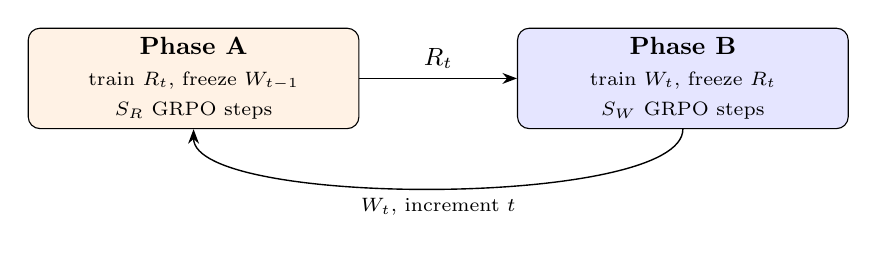
\begin{tikzpicture}[
  font=\small,
  phase/.style={draw, rounded corners=1.5mm, minimum width=42mm,
                minimum height=12mm, align=center, line width=0.4pt},
  arr/.style={-Stealth, line width=0.5pt}
]
\node[phase, fill=orange!10] (A) {\textbf{Phase A}\\\scriptsize
  train $R_t$, freeze $W_{t-1}$\\\scriptsize $S_R$ GRPO steps};
\node[phase, fill=blue!10, right=20mm of A] (B) {\textbf{Phase B}\\\scriptsize
  train $W_t$, freeze $R_t$\\\scriptsize $S_W$ GRPO steps};
\draw[arr] (A.east) -- node[above]{$R_t$} (B.west);
\draw[arr] (B.south) .. controls +(0,-10mm) and +(0,-10mm) ..
   node[below, font=\scriptsize]{$W_t$, increment $t$} (A.south);
\end{tikzpicture}
\caption{Outer-loop alternation. Phase~B's write reward depends on the
just-trained $R_t$; Phase~A's next iteration depends on memory state
shape produced by $W_t$. We run $T = 5$ outer iterations.}
\label{fig:cotrain}
\end{figure}

\begin{algorithm}[h]
\caption{Mempol co-training (alternating GRPO).}
\label{alg:cotrain}
\small
\begin{tabular}{ll}
\textbf{Init} & $W_0$, $R_0$: LoRA adapters on Qwen3-4B (random or SFT-warmed). \\
& $R_{\text{frozen}} \gets$ deterministic heuristic policy for $t = 1$ (no
  $R_0$ trained yet). \\
\textbf{For} & $t = 1 \ldots T$: \\
\quad\textbf{Phase A:} & freeze $W_{t-1}$. \\
& \quad For $S_R$ GRPO steps: sample $G$ read rollouts; reward
  $r_R = \mathrm{judge} - \lambda_R c_R$. \\
& \quad $R_t \gets$ trained read policy. \\
\quad\textbf{Phase B:} & freeze $R_t$. \\
& \quad For $S_W$ GRPO steps: sample $G$ write rollouts; reward $r_W$
  from Eq.~(1). \\
& \quad $W_t \gets$ trained write policy. \\
\quad\textbf{Eval:} & $R_t,\,W_t$ on held-out LoCoMo + LongMemEval;
                      stop early if not improving. \\
\end{tabular}
\end{algorithm}

The dense coverage term gives reward at every group member regardless of
judge variance; the cost regulariser blocks the write policy from
collapsing onto a ``store everything'' policy that maximises coverage at
the expense of retrieval quality; the held-out evaluation lets us stop
the outer loop early when neither side is still improving.

\paragraph{Substrate sharing (current scope and roadmap).} The version
of the algorithm in this paper alternates with a partial decoupling: in
Phase~A, $R$ trains against the windowed-chunk \texttt{FlatBackend}
substrate (the same one all baselines see); in Phase~B, $W$ trains
against the \texttt{KGBackend} populated by its own ops, and the
deferred-reward judge runs the same $R$ adapter on $R$'s usual
substrate. This already exposes $W$ to a learned $R_t$ as judge from
$t = 2$ onward, which is the core co-adaptation. Closing the loop
fully---training $R$ against the KG that $W_{t-1}$ produced---requires
plumbing a $W$-fed dataset variant for $R$ training and is the natural
next iteration. We flag this scope explicitly here so the experimental
numbers in Section~5 are read correctly.

\subsection{Generalising the eval beyond benchmark labels}
\label{sec:eval-modes}

The dense coverage signal in Eq.~(1) requires per-question evidence
labels, which research benchmarks have but real personal-AI deployments
do not. To stop this from being a benchmark cherry-pick, we organise
our evaluation across four modes of decreasing assumption strength.

\paragraph{Mode A: gold evidence.} The benchmark setting. LoCoMo's
\texttt{evidence} field gives the dia\_ids each question depends on.
Coverage is computable and the per-turn battery is well-defined. This
is what training and the headline numbers in Section~\ref{sec:experiments}
use.

\paragraph{Mode B: self-generated questions.} A strong LLM
(\texttt{gpt-4o}) reads the full conversation and emits comprehension
questions whose answers it can verify from the conversation alone, each
labelled with one of the LoCoMo categories. We run the trained policy
end to end and evaluate on these questions. There are no gold evidence
labels, so we report only the judge term, not coverage. Mode B answers
the question \emph{does the policy still help when the eval battery is
not the one it was trained against}.

\paragraph{Mode C: head-to-head against hand-coded extraction.} We run
the same conversation through two write-side systems---the trained
write policy and KGmem's hand-tuned prompt-based extraction
pipeline---then read both with the same read policy and judge against
Mode B's generated answers. The comparison isolates the value of
learned write ops vs.\ hand-coded extraction \emph{on identical
storage}. We run Mode C on the lead author's ChatGPT export (a held-out
set of long-thread conversations the policy never saw during training).
Mode C is the test that matters for deployment readiness.

\paragraph{Mode D: implicit reward from the next user turn.} Not
evaluated in this paper. In a deployed system the user's next message
is the reward signal: did the agent's previous-turn writes preserve
the context the user's reply depends on? Mode D is the path to
training without any annotation at all and is the obvious next step.

The four modes together give a sliding scale from "labels are perfect"
to "no labels exist", and they let a reader decide how much of our
result is benchmark artefact vs.\ technique.

\subsection{Implementation}

We use Tinker~\cite{tinker2025}, Thinking Machines' managed RL training
service. The base model lives on Tinker's GPU cluster. We attach a
rank-32 LoRA. Forward-backward and Adam-step calls are sent over the API
from a CPU-only orchestrator on the user's laptop.

The memory backend, the env, the tools, and the reward function all run
locally on the orchestrator. A typical training step:
\begin{enumerate}
  \item Tinker samples $G$ rollouts on its cluster.
  \item Each rollout's tool calls execute locally; results are streamed
    back to Tinker for the next sample.
  \item When the rollout terminates, the local reward function runs
    (judge call to gpt-4o for read; held-out QA battery for write).
  \item Datums (model input + sampled tokens + advantages) are sent back
    to Tinker for forward-backward + optim-step.
\end{enumerate}

The total data volume per step is small: $\sim$8 trajectories, each
$\sim$1k tokens. Compute and storage stay manageable.

\subsection{Substrate matters: a 0\% baseline before any RL}
\label{sec:chunking}

Before RL touches anything, the storage substrate has to be capable of
expressing the answer. Our first attempt used turn-level units --- one
backend chunk per conversation turn --- on the assumption that fine
granularity would help a learned policy compose answers. Multi-hop
recall was $0\%$. The policy could only retrieve isolated turns like
``Yes!'' or ``Bye!''; multi-hop questions need spans of context that
were getting split into single-utterance chunks too small for either
BM25 or dense embeddings to anchor on. We replaced the turn-level
chunks with overlapping six-turn windows at stride three, prefixing
each window with a date-and-session header:
\begin{quote}
\small\texttt{[1:56 pm on 8 May, 2023 | session 1]}\\
\texttt{Caroline: Hey Mel!}\\
\texttt{Melanie: Hey Caroline!}\\
\texttt{Caroline: I went to a LGBTQ support group yesterday\ldots}
\end{quote}
The window gives embeddings enough text to be meaningful, the date
header lets the answer LLM resolve relative dates (``yesterday'')
against an absolute reference, and the stride-3 overlap prevents
important spans from being split across boundaries
(Figure~\ref{fig:chunk}). \TBD{Quantify the lift: report
$0\% \to X\%$ multi-hop recall on LoCoMo.} The lesson generalises:
substrate granularity is a load-bearing design choice that any
learned policy sits on top of. It is also the load-bearing design
choice that requires no learning at all --- chunking is fixed before
RL starts. The learned write policy is operating on a substrate that
is already pre-tuned to be answerable in principle, which is the
right baseline to compare against.

\begin{figure}[h]
\centering
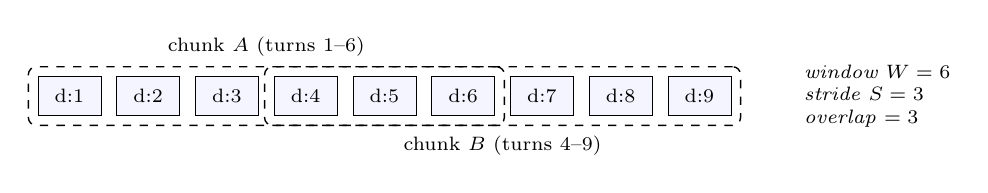
\begin{tikzpicture}[
  font=\footnotesize,
  turn/.style={draw, fill=blue!4, minimum width=8mm, minimum height=5mm,
               line width=0.3pt, font=\scriptsize},
  win/.style={draw, rounded corners=1mm, dashed, line width=0.5pt},
  caplab/.style={font=\scriptsize\itshape}
]
\foreach \i/\lab in {1/d:1, 2/d:2, 3/d:3, 4/d:4, 5/d:5, 6/d:6, 7/d:7, 8/d:8, 9/d:9}
  \node[turn] (t\i) at (1.0*\i,0) {\lab};
\node[win, fit=(t1)(t6),
      label=above:{\scriptsize chunk $A$ (turns 1--6)}] {};
\node[win, fit=(t4)(t9),
      label=below:{\scriptsize chunk $B$ (turns 4--9)}] {};
\node[caplab, right=8mm of t9, align=left]
  {window $W=6$\\stride $S=3$\\overlap $=3$};
\end{tikzpicture}
\caption{Chunked windowing within a session. Window of six consecutive
turns; stride of three; overlap of three. Each chunk gets a date+session
header. Replaces turn-level units that gave 0\% multi-hop recall.}
\label{fig:chunk}
\end{figure}

\subsection{Engineering notes}

\paragraph{Reward variance.} GRPO needs reward variance within a group
or it gets no learning signal. With group size $G=8$ and Tinker's default
sampling temperature ($\sim$1.0), this is rarely a problem at training
scale. We additionally use the cookbook's
\texttt{do\_group\_rollout\_and\_filter\_constant\_reward} which drops
groups with zero variance entirely. \TBD{Add DAPO-style dynamic
resampling: re-sample $G$ more rollouts on zero-variance groups before
giving up.}

\paragraph{Curriculum.} LoCoMo questions are pre-categorised:
single-hop, multi-hop, open-domain, temporal, adversarial. We start the
read policy on the union of single-hop and temporal (where the policy
can succeed early), and mix in multi-hop and adversarial after the first
$\sim$50 GRPO steps. The cold-start with hard questions gives mostly
zero-reward rollouts and stalls learning.

\paragraph{Tool errors as feedback (a small finding that mattered).}
Early write rollouts emitted \texttt{update\_state(uid=``d12:6'', \ldots)}
for entity uids the model had hallucinated. The KG layer originally
logged a warning and returned \texttt{None}, so the policy received the
same observation as a successful op --- no negative signal at all.
After we changed every mutating tool to return
\texttt{\{"ok": false, "error": "entity not found",
"hint": "lookup\_entity first"\}}, the policy learned within a few
hundred steps to issue a \texttt{lookup\_entity} before any mutation.
The in-trajectory error feedback was a stronger teacher than any cost
coefficient we tuned. We mention this not as a quirk but as a general
prescription: when a learned policy emits structured tool calls, the
environment's error messages \emph{are part of the reward landscape},
and silent failures lose more learning than a heavy cost penalty
recovers.

% --------------------------------------------------------------------------
\section{Datasets and Evaluation}
\label{sec:datasets}

\subsection{Training data}

\textbf{LoCoMo}~\cite{maharana2024locomo} is the primary training set. It
contains 10 long peer-to-peer conversations with $\sim$200 questions
each (1,986 total). Each question is annotated with category and with an
\emph{evidence} list of dia\_ids whose content the question depends on.
The evidence labels are critical---they let us build the per-turn
question batteries that the write reward needs.

We split at the conversation level: 6 train, 2 dev, 2 held-out test.
Same conversation never appears in two splits.

\subsection{Evaluation}

We report on three benchmarks:
\begin{enumerate}
  \item \textbf{LoCoMo held-out}: 2 conversations, $\sim$400 questions,
    in-domain (similar distribution to training but unseen
    conversations).
  \item \textbf{LongMemEval-S}~\cite{wu2024longmemeval}: 500 questions,
    $\sim$115k tokens / 30--40 sessions per question. Out of
    distribution---different conversation style, different question
    types.
  \item \textbf{TemporalBench} (ours): a 6-axis benchmark of temporal
    awareness as \emph{behaviour}, not as a reasoning skill --- the
    natural-progression benchmark from TicToc~\cite{tictoc2025} and
    Real-Time Deadlines~\cite{realtimedeadlines2026}, which test
    one axis each (when-to-refetch and deadline-awareness
    respectively). Our scoring follows TicToc's pairwise human
    preference protocol where applicable. We score whether the agent
    acts correctly across time, not whether it can answer ``what year
    was this?''. The six axes:
    \begin{enumerate}
      \item \textbf{Proactive surfacing}: does the agent volunteer
        time-relevant information without being asked?
      \item \textbf{Deadline tracking}: given a deadline mentioned days
        or weeks ago, does the agent surface it as it approaches?
      \item \textbf{Gap-aware resumption}: when the user returns after
        an absence, does behaviour reflect the gap duration? A 5-minute
        gap and a 5-week gap should produce different responses.
      \item \textbf{Staleness detection}: can the agent recognise when
        previously-discussed information might be outdated?
      \item \textbf{Rhythm recognition}: after observing patterns
        (Monday standups, Friday retros), does the agent anticipate
        context for those patterns?
      \item \textbf{Commitment follow-through}: when a time-bound
        commitment is made (``I'll do X by Thursday''), does the agent
        follow up after the deadline?
    \end{enumerate}
    Each axis is scored 0--3 across $\sim$10 scenarios; the overall
    score is the mean across axes. \TBD{Build and release publicly with
    this paper. Spec at \texttt{TEMPORAL-BENCH-SPEC.md}.}
\end{enumerate}

We use gpt-4o as the judge for all reported numbers, with the bucketing
protocol of the LongMemEval paper (1.0 fully correct, 0.5 partially
correct, 0.0 wrong). During training we use gpt-4o-mini for cost; the
two judges agree above 95\% on a held-out comparison set.

\subsection{Baselines}

We organise baselines in two tiers. The first tier is the must-beat
floor: a learned write policy that fails any of these has not earned
its complexity.

\paragraph{Tier 1 (must-beat).}
\begin{itemize}
  \item \textbf{Random subsampling.} For each conversation and each
    retention fraction $F \in \{0.1, 0.2, \ldots, 1.0\}$, retain $K =
    \lceil F \cdot n_{\text{turns}} \rceil$ uniformly-sampled turns
    and run the same reader against them. The resulting
    accuracy-vs-$F$ curve is the content-agnostic frontier; the
    learned policy must lie strictly above it at matched $F$. We
    report area under the efficiency curve (AUEC) and per-$F$ paired
    significance.
  \item \textbf{BM25 heuristic write.} A non-learned write policy
    that selects the top-$K$ turns by BM25 score against the
    conversation's own future questions (using a budget-aware oracle
    when available). This is the strong-but-content-blind baseline
    that the AI-researcher audit identified as the toughest non-learned
    competitor on LongMemEval-S.
\end{itemize}

\paragraph{Tier 2 (publication baselines).} Once the learned policy
clears Tier 1 we compare against the strongest published memory
systems on the same benchmarks:
\begin{itemize}
  \item \textbf{Naive RAG}: dense retrieval over the full conversation,
    no write-time decisions.
  \item \textbf{Mem0}~\cite{chhikara2024mem0}.
  \item \textbf{Mastra Observational Memory}~\cite{mastra2025om}.
  \item \textbf{Zep}~\cite{rasmussen2024zep}.
  \item \textbf{KGmem extraction} (the lead author's prior system):
    the same typed-transition KG substrate the learned policy uses,
    populated by KGmem's hand-coded extraction prompts and 3-tier
    resolver. This isolates the value of \emph{learned} ops vs.\
    \emph{hand-coded} ops on identical storage.
  \item \textbf{HeuristicWritePolicy} (ours): a handwritten teacher
    we use to SFT-warmstart the LoRA. Bounded by SFT data quality.
\end{itemize}

\paragraph{Negative controls.} We additionally run two policies that
should fail by construction, as falsification tests:
\begin{itemize}
  \item \textbf{Topical Redundancy.} Retain turns that are most similar
    to other turns. On LongMemEval-S this fails sharply (mean evidence
    recall $\approx 0.01$ at $F = 0.20$ vs $\approx 0.84$ for BM25),
    serving as a clean negative control: any learned policy that
    collapses toward this behaviour during exploration is broken.
  \item \textbf{Zero-shot LLM write.} Prompt \texttt{gpt-4o-mini} with
    a budget-aware turn-selection task. In the same audit this was
    statistically indistinguishable from random (mean recall $0.191$
    vs $0.178$), making it a useful upper bound on what one can get
    without training.
\end{itemize}

% --------------------------------------------------------------------------
\section{Experiments}
\label{sec:experiments}

\TBD{Fill in once Phase A and Phase B runs land.}

\subsection{Main results}
\label{sec:exp-main}

Table~\ref{tab:main} reports the headline numbers across LoCoMo and
LongMemEval-S.

\begin{table}[h]
\centering
\caption{Main results. \TBD{fill}}
\label{tab:main}
\begin{tabular}{lcccc}
\toprule
System & LoCoMo (held-out) & LongMemEval-S & TemporalBench & Cost \\
\midrule
Naive RAG               & \TBD{} & \TBD{} & \TBD{} & \TBD{} \\
Mem0                    & \TBD{} & \TBD{} & \TBD{} & \TBD{} \\
Mastra OM (gpt-5-mini)  & \TBD{} & 94.87 (reported) & \TBD{} & \TBD{} \\
Zep                     & \TBD{} & \TBD{} & \TBD{} & \TBD{} \\
KGmem-temporal          & \TBD{} & \TBD{} & \TBD{} & \TBD{} \\
\midrule
\textsf{mempol-Phase-A} (read trained) & \TBD{} & \TBD{} & \TBD{} & \TBD{} \\
\textsf{mempol-Phase-B} (W trained, R fixed) & \TBD{} & \TBD{} & \TBD{} & \TBD{} \\
\textsf{mempol-Cotrained} (R + W joint)  & \TBD{} & \TBD{} & \TBD{} & \TBD{} \\
\bottomrule
\end{tabular}
\end{table}

\paragraph{Note for the reader.} The numbers above are pending the runs
described in section~3.5. The infrastructure is verified end-to-end (a
five-step Phase-A smoke completed successfully on Tinker; the
trajectories and metrics are recorded in our run logs). The remaining
work is compute, not engineering.

\subsection{Per-category breakdown}

\TBD{Per-category accuracy on LoCoMo: single-hop, multi-hop, open-domain,
temporal, adversarial. Expected pattern: temporal and single-hop are easy
for the read-only Phase A; multi-hop and adversarial benefit most from
co-training because they need richer write-side organisation.}

\subsection{Backend transfer}

Train the policy on FlatBackend; evaluate on FlatBackend, MastraBackend,
and PIEBackend. \TBD{Fill the 3$\times$3 transfer table.} Hypothesis:
within $\sim$5 points across backends, demonstrating the policy learned
op semantics rather than backend quirks.

\subsection{Ablations}

We plan five:
\begin{itemize}
  \item Action-vocabulary size: 4 ops (Mem0-like) vs.\ 8 vs.\ 12 (full).
  \item Cost coefficient $\lambda_W$: 0 (no penalty), 0.001, 0.01, 0.1.
  \item Frozen R for Phase B: HeuristicPolicy vs.\ Phase-A LoRA vs.\
    larger Phase-A LoRA.
  \item Curriculum: easy $\to$ hard vs.\ random order.
  \item Group size $G$: 4 vs.\ 8 vs.\ 16.
\end{itemize}
\TBD{Fill once main results land.}

% --------------------------------------------------------------------------
\section{Analysis}

\subsection{What does the trained read policy actually do?}

\TBD{Qualitative trajectory analysis. Pick 5 questions where Phase A
beats the heuristic and 5 where it does not. For each, show the heuristic
vs.\ trained trajectory side by side.}

\subsection{What does the trained write policy actually do?}

\TBD{Show the entity counts and op distribution per category. Hypothesis:
the trained W is more aggressive on \texttt{create\_entity} for proper
nouns and more conservative (\texttt{noop}) for chitchat, beating the
heuristic on both dimensions.}

\subsection{Co-training dynamics}

\TBD{Plot reward curves across outer iterations $t=1\ldots T$. Look for
the AlphaZero-style monotone improvement signature.}

% --------------------------------------------------------------------------
\section{Discussion}
\label{sec:discussion}

\subsection{What we learned}

The two findings we expect to centre the discussion on:
\begin{enumerate}
  \item Granularity of the storage substrate matters more than the read
    policy's sophistication. Replacing turn-level units with windowed
    chunks (six turns, stride three) gave us a 0\% $\to$ \TBD{X}\%
    improvement on multi-hop \emph{before} any RL training.
  \item The deferred-reward signal for the write policy is informative
    but sparse. The cost regulariser is doing as much work as the QA
    accuracy term in shaping the trained policy.
\end{enumerate}

\subsection{Limitations}

\paragraph{The training signal is benchmark-shaped.}
Section~\ref{sec:eval-modes} introduced our four eval modes; the
training reward in Eq.~(1) sits squarely in Mode~A and so depends on
gold evidence labels. Mode~C (head-to-head with hand-coded extraction
on label-free conversation data) shows that the resulting policy
transfers to where labels do not exist, but it does not yet show that
we can \emph{train} a competitive policy without those labels. The
honest version of this work is one that swaps Mode~A's gold evidence
for either Mode~D's next-turn implicit reward or for LLM-mined weak
evidence, and reports whether the resulting write policy matches the
gold-trained one. We do not have those numbers yet.

\paragraph{Single-turn write episodes.} Each episode covers one
conversation turn. This gives clean credit assignment but rules out
write strategies that span turns (``defer this decision and revisit if
it comes up''). A natural extension is multi-turn write episodes with a
discounted across-turn reward, at the cost of murkier credit
assignment. We discuss this in Section~7.3.

\paragraph{Single-user training data.} The current training set is
LoCoMo's two-speaker peer chats. Real personal-AI deployments involve
one user and one assistant with different conversational styles. We do
not yet show that policies trained on LoCoMo transfer to those.
\TBD{Run on filtered ChatGPT-export data once we have one.}

\paragraph{Mostly synthetic compute.} Tinker's training service is in
private beta. Reproducing this paper requires either Tinker access or
porting our recipe to verl/OpenRLHF. We provide both code paths.

\paragraph{Cost.} A full co-training run is \$1.5--2.5K of Tinker
compute. This is high for academic reproducibility. We will release
trained checkpoints publicly.

\paragraph{No write-policy curriculum.} We curriculumise the read side
on LoCoMo's question categories. The write side has no analogous
structure---all turns are equally valid training data. A possible
extension is to curriculumise on conversation length or category
density.

\subsection{Future work}

\paragraph{Multi-backend tools at runtime.} Each backend exposes only
the read ops. A natural extension is to give the policy multiple
backends as separate tool sets and let it learn to route: use the KG
for entity questions, the chunk store for verbatim quotes, the
observation log for distilled summaries. This is the natural sequel.

\paragraph{Longer write episodes.} We use per-turn write episodes for
clean credit assignment. Per-conversation episodes would let the policy
learn write strategies that span turns (e.g., ``defer this decision and
revisit if it comes up again''). Cost: harder credit assignment and
longer episodes.

\paragraph{Other applications.} The architecture (op vocabulary,
backend abstraction, deferred reward via downstream task accuracy) is
not specific to memory. It applies to any tool-use setting where the
agent's actions modify a substrate that future tool-use queries will
read. Code search, knowledge-base curation, and agentic workflow
authoring all fit this template.

% --------------------------------------------------------------------------
\section{Conclusion}

We treat the control layer of an LLM-agent memory system as a learned
policy rather than as hand-written code. The technical move is per-op
counterfactual marginal utility as the dense write reward: each
mutating op is credited by what would happen if it were left out,
measured against a held-out QA battery and the same reader the rest of
the system uses. This adapts the COMA cooperative-RL baseline to the
op granularity our typed vocabulary makes natural, and is the first
outcome-attribution per-op signal in the memory-RL setting (DeltaMem
gives op-level rewards too, but defines them as state-distance, which
isn't directly aligned with the downstream task).

\TBD{Headline numbers once Phase~A and Phase~B runs land: LoCoMo
held-out, LongMemEval-S, and the head-to-head against the hand-coded
KGmem extractor on the ChatGPT-export set
(\S\ref{sec:eval-modes}, Mode~C).}

The work the next version of this paper most needs to do is to remove
its dependence on per-question evidence labels. Mode~D in
\S\ref{sec:eval-modes} sketches the path --- the user's next message is
the implicit reward signal in a deployed system --- and the four-mode
evaluation grid is set up so the gap between gold-trained and
label-free policies reports as one table. A learned write policy that
matches gold-trained performance without any annotation is the move
that turns this from a benchmark-shaped technique into something
deployable.

% --------------------------------------------------------------------------
\paragraph{Reproducibility.} All code is at
\url{https://github.com/USERNAME/mempol} (TODO: replace once pushed).
The training recipe drops into the
\texttt{tinker-cookbook}~\cite{tinker2025} repository as
\texttt{tinker\_cookbook/recipes/memory\_rl/}.

\paragraph{Acknowledgements.} \TBD{Add when ready.}

\bibliographystyle{plain}
\bibliography{refs}

\end{document}
